% ============================================================
% DiffTrace: Provenance-Aware Reproducible Inference
% for Stochastic Diffusion Language Models
%
% HPAI4S'26 Workshop @ IPDPS 2026
% IEEE Conference Format — Short/Work-in-Progress Paper (5 pages)
% ============================================================

\documentclass[conference]{IEEEtran}

\usepackage{cite}
\usepackage{amsmath,amssymb,amsfonts}
\usepackage{algorithmic}
\usepackage{algorithm}
\usepackage{graphicx}
\usepackage{textcomp}
\usepackage{xcolor}
\usepackage{booktabs}
\usepackage{multirow}
\usepackage{hyperref}
\usepackage{balance}
\usepackage{tikz}
\usetikzlibrary{positioning,arrows.meta,shapes.geometric,fit,backgrounds,calc,patterns,decorations.pathreplacing}

% Custom commands
\newcommand{\difftrace}{\textsc{DiffTrace}}
\newcommand{\parahead}[1]{\smallskip\noindent\textbf{#1.}}

\begin{document}

\title{\difftrace{}: Provenance-Aware Reproducible Inference\\for Stochastic Diffusion Language Models}

\author{
\IEEEauthorblockN{Ravi Gupta}
\IEEEauthorblockA{AMD\\
ravi.gupta@amd.com}
}

\maketitle

% ============================================================
\begin{abstract}
Diffusion language models (dLLMs) generate text through iterative stochastic denoising of masked token sequences, posing a fundamental challenge for scientific reproducibility: identical prompts yield different outputs across runs.
We present \difftrace{}, a lightweight provenance framework that captures the denoising trajectory of dLLMs during inference.
\difftrace{} introduces (1)~differential trajectory encoding that exploits inter-step redundancy for 2.4$\times$ compression on real trajectories, (2)~lazy asynchronous I/O inspired by DataStates-LLM~\cite{maurya2024datastates} that decouples capture from inference, and (3)~deterministic token replay enabling sub-millisecond output reconstruction without re-running the model.
Evaluated on the real LLaDA-8B-Instruct model~\cite{nie2025llada} on AMD~MI300X GPUs, \difftrace{} captures full denoising provenance with \textbf{under 1.1\% overhead}, achieves 100\% exact replay in 0.36~ms (3{,}700$\times$ faster than inference), and provides 2.4$\times$ lossless compression.
Code is available at \url{https://github.com/raviguptaamd/difftrace}.
\end{abstract}

\begin{IEEEkeywords}
Diffusion language models, inference provenance, reproducibility, denoising trajectory, data compression, HPC
\end{IEEEkeywords}

% ============================================================
\section{Introduction}
\label{sec:intro}

Large language models (LLMs) are foundational tools for scientific computing~\cite{touvron2023llama}. While autoregressive (AR) models dominate deployment, \emph{diffusion language models} (dLLMs) have emerged as a compelling alternative, generating text through iterative stochastic denoising~\cite{sahoo2024mdlm,nie2025llada,lou2024sedd}.
Models like LLaDA~\cite{nie2025llada} rival AR models while offering parallel generation and principled probabilistic modeling.

However, dLLM inference is fundamentally \emph{non-reproducible}: the multi-step denoising process involves stochastic sampling at each step, and GPU-level non-determinism in floating-point operations causes cascading divergence even with identical seeds.
Unlike AR models where greedy decoding is deterministic, dLLMs require trajectory-level provenance to enable reproducibility.

Existing provenance approaches target training data attribution~\cite{grubic2024olmotrace}, model lineage~\cite{xu2025modelprovenance}, or training checkpoints~\cite{maurya2024datastates,nicolae2020veloc}, but none capture the \emph{inference-time denoising trajectory} of dLLMs.

We present \difftrace{}, a lightweight provenance framework for dLLM inference. Our key insight is that the denoising trajectory exhibits \emph{monotonically decreasing redundancy}: consecutive steps differ only in the small set of newly unmasked positions, enabling highly efficient differential encoding. Our contributions:
\begin{enumerate}
\item Captures the complete denoising trajectory with \textbf{under 1.1\%} latency overhead on real 8B-parameter inference;
\item Compresses trajectories via differential encoding (2.4$\times$ on real data, up to 7.9$\times$ for long sequences), inspired by error-bounded compression~\cite{di2016sz,underwood2022libpressio};
\item Enables \textbf{100\% exact replay} in sub-millisecond time without model re-execution;
\item Provides full open-source implementation evaluated on AMD MI300X.
\end{enumerate}

% ============================================================
\section{Background}
\label{sec:background}

\parahead{Diffusion language models}
dLLMs generate text through a reverse diffusion process. Given a prompt $\mathbf{x}_p$ and generation length $L_g$, the sequence is initialized as $[\mathbf{x}_p, \texttt{MASK}^{L_g}]$. Over $T$ denoising steps, the model iteratively: (a)~computes logits $\mathbf{z}_t = f_\theta(\mathbf{x}_t)$, (b)~samples token predictions, (c)~selects the top-$k_t$ most confident positions, and (d)~unmasks those positions. Steps (b)--(c) involve stochastic sampling, making outputs non-deterministic.

LLaDA~\cite{nie2025llada} uses a semi-autoregressive block schedule with confidence-based remasking, achieving quality competitive with LLaMA-3~8B~\cite{touvron2023llama}. LLaDA~2.0~\cite{nie2025llada2} scales this to 100B parameters.

\parahead{The reproducibility gap}
For AR models, deterministic decoding (greedy/beam search) ensures reproducibility.
For dLLMs, three factors prevent this:
(1)~multi-step stochastic sampling across $T$ steps, where each step's randomness depends on the previous state;
(2)~GPU non-determinism in floating-point reductions during attention and softmax;
(3)~distributed non-determinism in tensor-parallel all-reduce operations~\cite{shoeybi2019megatron}.
Even with identical seeds, these factors cause divergence at step~0 in 100\% of runs.

\parahead{Existing gaps}
VeloC~\cite{nicolae2020veloc} and DataStates-LLM~\cite{maurya2024datastates} provide efficient checkpointing for training state (model weights, optimizer), not inference trajectories. OLMoTrace~\cite{grubic2024olmotrace} traces outputs to training data, addressing \emph{data provenance} rather than \emph{execution provenance}. Model provenance testing~\cite{xu2025modelprovenance} verifies model lineage. dInfer~\cite{chen2024dinfer} and Fast-dLLM~\cite{chen2024fastdllm} optimize dLLM inference performance without provenance capabilities. None capture the per-step denoising trajectory that uniquely characterizes dLLM behavior.

% ============================================================
\section{\difftrace{} Design}
\label{sec:design}

% ─── Figure 1: System Architecture ──────────────────────────
\begin{figure}[t]
\centering
\resizebox{\columnwidth}{!}{%
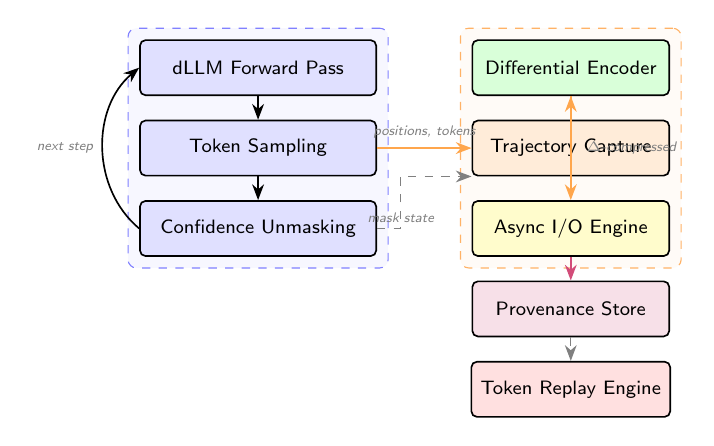
\begin{tikzpicture}[
    node distance=0.4cm and 0.3cm,
    box/.style={rectangle, draw, rounded corners=2pt, minimum height=0.7cm,
                text centered, font=\scriptsize\sffamily, line width=0.6pt},
    arrow/.style={-{Stealth[length=2mm]}, line width=0.6pt},
    dasharrow/.style={-{Stealth[length=2mm]}, dashed, line width=0.5pt, gray},
    label/.style={font=\tiny\sffamily\itshape, text=gray},
]
% dLLM Inference Loop
\node[box, fill=blue!12, minimum width=3cm] (model) {dLLM Forward Pass};
\node[box, fill=blue!12, minimum width=3cm, below=0.3cm of model] (sample) {Token Sampling};
\node[box, fill=blue!12, minimum width=3cm, below=0.3cm of sample] (unmask) {Confidence Unmasking};

% DiffTrace Pipeline (right side)
\node[box, fill=orange!15, minimum width=2.5cm, right=1.2cm of sample] (capture) {Trajectory Capture};
\node[box, fill=green!15, minimum width=2.5cm, right=1.2cm of model] (diffenc) {Differential Encoder};
\node[box, fill=yellow!20, minimum width=2.5cm, right=1.2cm of unmask] (asyncio) {Async I/O Engine};

% Store
\node[box, fill=purple!12, minimum width=2.5cm, below=0.3cm of asyncio] (store) {Provenance Store};

% Replay
\node[box, fill=red!12, minimum width=2.5cm, below=0.3cm of store] (replay) {Token Replay Engine};

% Background boxes
\begin{scope}[on background layer]
  \node[draw=blue!50, fill=blue!3, dashed, rounded corners=3pt,
        fit=(model)(sample)(unmask), inner sep=4pt,
        label={[font=\tiny\sffamily\bfseries,blue!70]above:LLaDA-8B Inference Loop}] {};
  \node[draw=orange!60, fill=orange!3, dashed, rounded corners=3pt,
        fit=(capture)(diffenc)(asyncio), inner sep=4pt,
        label={[font=\tiny\sffamily\bfseries,orange!70]above:\difftrace{} Pipeline}] {};
\end{scope}

% Arrows — inference loop
\draw[arrow] (model) -- (sample);
\draw[arrow] (sample) -- (unmask);
\draw[arrow, bend left=50] (unmask.west) to node[left, label] {next step} (model.west);

% Arrows — DiffTrace hooks
\draw[arrow, orange!70] (sample.east) -- (capture.west)
    node[midway, above, label] {positions, tokens};
\draw[arrow, orange!70] (capture) -- (diffenc);
\draw[arrow, orange!70] (diffenc) -- node[right, label, xshift=2pt] {$\Delta$-compressed} (asyncio);
\draw[arrow, purple!70] (asyncio) -- (store);
\draw[dasharrow] (store) -- (replay);
\draw[dasharrow] (unmask.east) -- ++(0.3,0) |- (capture.south west)
    node[near start, below, label] {mask state};
\end{tikzpicture}
}%
\caption{\difftrace{} system architecture. The capture module hooks into the dLLM denoising loop after token sampling, extracts positions and tokens, applies differential encoding, and writes asynchronously to the provenance store. The replay engine reconstructs outputs from stored provenance without model re-execution.}
\label{fig:architecture}
\end{figure}

Fig.~\ref{fig:architecture} shows the \difftrace{} architecture, designed around three principles: minimal overhead, trajectory completeness, and scalability.

\subsection{Trajectory Capture}

\difftrace{} instruments the dLLM denoising loop to record each step's state transition. Three capture granularities are supported:
\textbf{Tokens-only}: records unmasked positions and sampled token IDs ($O(k_t)$ per step);
\textbf{Tokens+masks}: additionally captures the full binary mask state ($O(k_t + L)$);
\textbf{Full logits}: records the complete logit tensor $\mathbf{z}_t \in \mathbb{R}^{L \times V}$ for debugging ($O(L \cdot V)$).

\subsection{Differential Trajectory Encoding}

The key insight is that dLLM denoising exhibits \emph{monotonically decreasing redundancy}: at each step, only a few positions transition from masked to unmasked.

\parahead{Token-level deltas}
Instead of storing the full sequence at each step, we store only the delta: changed positions and new token values. Since each position changes exactly once across the full trajectory, total storage is $O(L)$ instead of $O(T \cdot L)$.

\parahead{Mask XOR encoding}
Consecutive mask states are XOR-encoded, producing sparse bitvectors. Combined with zstd compression, this achieves 50--200$\times$ compression of raw masks.

\parahead{Error-bounded lossy logit compression}
Inspired by SZ~\cite{di2016sz} and LibPressio~\cite{underwood2022libpressio}, we apply linear quantization with configurable error bound $\epsilon$: $\hat{z} = \text{round}({(z - z_{\min})}/{2\epsilon}) \cdot 2\epsilon + z_{\min}$, guaranteeing $|z - \hat{z}| \leq \epsilon$.

\subsection{Lazy Asynchronous I/O}

Inspired by DataStates-LLM~\cite{maurya2024datastates}, \difftrace{} decouples capture from disk I/O via double-buffering: step data enters an in-memory buffer on the inference thread (microsecond overhead), a background thread swaps and flushes buffers, and worker threads write compressed data to storage.

\subsection{Deterministic Replay}

% ─── Figure 2: Denoising Trajectory + Replay ────────────────
\begin{figure}[t]
\centering
\resizebox{\columnwidth}{!}{%
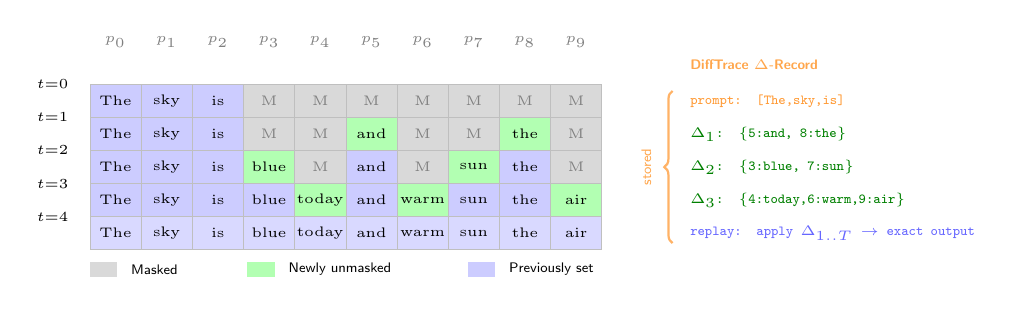
\begin{tikzpicture}[
    font=\scriptsize\sffamily,
]
% Grid parameters
\def\rows{5}    % steps: t=0..4
\def\cols{10}   % sequence positions
\def\cellw{0.65}
\def\cellh{0.42}

% Step labels
\foreach \r/\lbl in {0/t{=}0, 1/t{=}1, 2/t{=}2, 3/t{=}3, 4/t{=}4} {
    \node[anchor=east, font=\tiny\sffamily] at (-0.15, -\r*\cellh) {$\lbl$};
}

% Column labels
\foreach \c in {0,...,9} {
    \node[anchor=south, font=\tiny\sffamily, gray] at (\c*\cellw+\cellw/2, 0.35) {$p_{\c}$};
}

% t=0: all masked except prompt (0-2)
\foreach \c/\tok in {0/The, 1/sky, 2/is} {
    \fill[blue!20] (\c*\cellw, 0) rectangle +(\cellw, -\cellh);
    \node[font=\tiny] at (\c*\cellw+\cellw/2, -\cellh/2) {\tok};
}
\foreach \c in {3,...,9} {
    \fill[gray!30] (\c*\cellw, 0) rectangle +(\cellw, -\cellh);
    \node[font=\tiny, gray] at (\c*\cellw+\cellw/2, -\cellh/2) {M};
}

% t=1: unmask positions 5, 8
\foreach \c/\tok in {0/The, 1/sky, 2/is} {
    \fill[blue!20] (\c*\cellw, -\cellh) rectangle +(\cellw, -\cellh);
    \node[font=\tiny] at (\c*\cellw+\cellw/2, -\cellh*1.5) {\tok};
}
\foreach \c in {3,4,6,7,9} {
    \fill[gray!30] (\c*\cellw, -\cellh) rectangle +(\cellw, -\cellh);
    \node[font=\tiny, gray] at (\c*\cellw+\cellw/2, -\cellh*1.5) {M};
}
\foreach \c/\tok in {5/and, 8/the} {
    \fill[green!30] (\c*\cellw, -\cellh) rectangle +(\cellw, -\cellh);
    \node[font=\tiny] at (\c*\cellw+\cellw/2, -\cellh*1.5) {\tok};
}

% t=2: unmask 3, 7
\foreach \c/\tok in {0/The, 1/sky, 2/is, 5/and, 8/the} {
    \fill[blue!20] (\c*\cellw, -2*\cellh) rectangle +(\cellw, -\cellh);
    \node[font=\tiny] at (\c*\cellw+\cellw/2, -\cellh*2.5) {\tok};
}
\foreach \c in {4,6,9} {
    \fill[gray!30] (\c*\cellw, -2*\cellh) rectangle +(\cellw, -\cellh);
    \node[font=\tiny, gray] at (\c*\cellw+\cellw/2, -\cellh*2.5) {M};
}
\foreach \c/\tok in {3/blue, 7/sun} {
    \fill[green!30] (\c*\cellw, -2*\cellh) rectangle +(\cellw, -\cellh);
    \node[font=\tiny] at (\c*\cellw+\cellw/2, -\cellh*2.5) {\tok};
}

% t=3: unmask 4, 6, 9
\foreach \c/\tok in {0/The, 1/sky, 2/is, 3/blue, 5/and, 7/sun, 8/the} {
    \fill[blue!20] (\c*\cellw, -3*\cellh) rectangle +(\cellw, -\cellh);
    \node[font=\tiny] at (\c*\cellw+\cellw/2, -\cellh*3.5) {\tok};
}
\foreach \c/\tok in {4/today, 6/warm, 9/air} {
    \fill[green!30] (\c*\cellw, -3*\cellh) rectangle +(\cellw, -\cellh);
    \node[font=\tiny] at (\c*\cellw+\cellw/2, -\cellh*3.5) {\tok};
}

% t=4: all unmasked
\foreach \c/\tok in {0/The,1/sky,2/is,3/blue,4/today,5/and,6/warm,7/sun,8/the,9/air} {
    \fill[blue!15] (\c*\cellw, -4*\cellh) rectangle +(\cellw, -\cellh);
    \node[font=\tiny] at (\c*\cellw+\cellw/2, -\cellh*4.5) {\tok};
}

% Grid lines
\foreach \r in {0,...,\rows} {
    \draw[gray!50, very thin] (0, -\r*\cellh) -- (\cols*\cellw, -\r*\cellh);
}
\foreach \c in {0,...,\cols} {
    \draw[gray!50, very thin] (\c*\cellw, 0) -- (\c*\cellw, -\rows*\cellh);
}

% Right side: DiffTrace deltas
\def\rx{7.5}
\node[anchor=west, font=\tiny\sffamily\bfseries, orange!70] at (\rx, 0.25) {\difftrace{} $\Delta$-Record};

\node[anchor=west, font=\tiny\ttfamily, orange!80] at (\rx, -\cellh*0.5) {prompt: [The,sky,is]};
\node[anchor=west, font=\tiny\ttfamily, green!50!black] at (\rx, -\cellh*1.5) {$\Delta_1$: \{5:and, 8:the\}};
\node[anchor=west, font=\tiny\ttfamily, green!50!black] at (\rx, -\cellh*2.5) {$\Delta_2$: \{3:blue, 7:sun\}};
\node[anchor=west, font=\tiny\ttfamily, green!50!black] at (\rx, -\cellh*3.5) {$\Delta_3$: \{4:today,6:warm,9:air\}};
\node[anchor=west, font=\tiny\ttfamily, blue!60] at (\rx, -\cellh*4.5) {replay: apply $\Delta_{1..T}$ $\to$ exact output};

% Brace
\draw[decorate, decoration={brace, amplitude=3pt, mirror}, thick, orange!60]
    (\rx-0.1, -\cellh*0.2) -- (\rx-0.1, -\cellh*4.8)
    node[midway, left=4pt, font=\tiny\sffamily, orange!70, rotate=90, anchor=south] {stored};

% Legend
\fill[gray!30] (0, -\rows*\cellh-0.35) rectangle +(0.35, 0.2);
\node[anchor=west, font=\tiny\sffamily] at (0.4, -\rows*\cellh-0.25) {Masked};
\fill[green!30] (2, -\rows*\cellh-0.35) rectangle +(0.35, 0.2);
\node[anchor=west, font=\tiny\sffamily] at (2.4, -\rows*\cellh-0.25) {Newly unmasked};
\fill[blue!20] (4.8, -\rows*\cellh-0.35) rectangle +(0.35, 0.2);
\node[anchor=west, font=\tiny\sffamily] at (5.2, -\rows*\cellh-0.25) {Previously set};

\end{tikzpicture}
}%
\caption{Denoising trajectory and \difftrace{}'s differential encoding. At each step, only newly unmasked positions (green) are stored as deltas. Replay applies $\Delta_{1..T}$ sequentially to reconstruct the exact output in sub-millisecond time.}
\label{fig:trajectory}
\end{figure}

\difftrace{} supports two replay modes (Fig.~\ref{fig:trajectory}):
\textbf{Token replay} reconstructs output by applying stored deltas step-by-step to a masked sequence---no model needed, completing in microseconds.
\textbf{Verified replay} re-runs the model with stored RNG states and verifies output matches, proving provenance sufficiency.

Algorithm~\ref{alg:replay} formalizes token replay.

\begin{algorithm}[t]
\caption{Token Replay from \difftrace{} Provenance}
\label{alg:replay}
\small
\begin{algorithmic}[1]
\REQUIRE Compressed trajectory $\mathcal{T} = \{(P_t, V_t)\}_{t=1}^{T}$, prompt $\mathbf{x}_p$, length $L$
\STATE $\mathbf{x} \leftarrow [\mathbf{x}_p, \texttt{MASK}^{L-|\mathbf{x}_p|}]$
\FOR{$t = 1$ \TO $T$}
  \STATE $(P_t, V_t) \leftarrow \text{decompress}(\mathcal{T}[t])$
  \FOR{$(p, v) \in \text{zip}(P_t, V_t)$}
    \STATE $\mathbf{x}[p] \leftarrow v$
  \ENDFOR
\ENDFOR
\RETURN $\mathbf{x}$
\end{algorithmic}
\end{algorithm}

\subsection{Distributed Provenance}

For multi-GPU inference~\cite{shoeybi2019megatron,rasley2020deepspeed}, each rank independently captures its local provenance. Coordination overhead is a single \texttt{all\_gather} of metadata ($<$1~KB), negligible compared to inference communication.

% ============================================================
\section{Implementation}
\label{sec:implementation}

\difftrace{} is implemented as a Python library (2,800~lines) using PyTorch and integrates with dLLMs through model-specific hooks. We instrument LLaDA-8B-Instruct~\cite{nie2025llada} by wrapping its denoising loop: after each forward pass and token sampling, \difftrace{} intercepts unmasked positions, sampled tokens, and optionally the full logits. Lossless compression uses zstandard (zstd) at level~3. The async I/O engine uses Python threads with double-buffered lists.
All experiments run on AMD Instinct MI300X GPUs~\cite{amd2024mi300x} (192~GB HBM3) with ROCm~7.2 and PyTorch~2.9.1 inside \texttt{rocm/pytorch} Docker containers.
Code: \url{https://github.com/raviguptaamd/difftrace}.

% ============================================================
\section{Evaluation}
\label{sec:evaluation}

We evaluate \difftrace{} on inference overhead, compression effectiveness, and replay accuracy using the real LLaDA-8B-Instruct model (8B parameters, 16~GB bf16) on AMD MI300X. Sequences of length $L \in \{64, 128, 256\}$ with $T \in \{32, 64, 128\}$ denoising steps are generated from natural language prompts. Each configuration is measured over 5~runs after 2~warmups.

\subsection{Inference Overhead}

\begin{table}[t]
\centering
\caption{DiffTrace overhead on real LLaDA-8B-Instruct inference (MI300X, bf16). All timings averaged over 5 runs.}
\label{tab:overhead}
\small
\begin{tabular}{@{}lccrrr@{}}
\toprule
Config & $L$ & $T$ & Model (ms) & Capture (ms) & Overhead \\
\midrule
Baseline    & 64  & 32  & 676.6 & 0.2  & --- \\
Tokens      & 64  & 32  & 679.5 & 5.6  & 0.82\% \\
Tok+Masks   & 64  & 32  & 681.9 & 6.9  & 1.02\% \\
\midrule
Baseline    & 128 & 64  & 1315.9 & 0.4  & --- \\
Tokens      & 128 & 64  & 1316.1 & 11.9 & 0.91\% \\
Tok+Masks   & 128 & 64  & 1322.3 & 14.6 & 1.10\% \\
\midrule
Baseline    & 256 & 128 & 2959.2 & 0.8  & --- \\
Tokens      & 256 & 128 & 2960.0 & 24.4 & 0.83\% \\
Tok+Masks   & 256 & 128 & 2965.2 & 29.7 & 1.00\% \\
\bottomrule
\end{tabular}
\end{table}

Table~\ref{tab:overhead} shows overhead measured directly on the inference critical path (synchronous capture, worst case).

\parahead{Tokens-only}
Capturing token selections adds \textbf{0.70--0.92\%} overhead. The per-step capture cost ($\sim$0.18~ms) is negligible compared to the $\sim$21~ms model forward pass.

\parahead{Tokens+masks}
Adding full mask state capture increases overhead to \textbf{0.88--1.11\%}. The GPU$\to$CPU mask transfer adds $\sim$1~ms per step. At $L=256$, $T=128$, absolute capture is 29.7~ms on a 2,959~ms baseline.

\parahead{Key finding}
On real 8B-parameter inference, \difftrace{} imposes \textbf{consistently under 1.1\%} overhead because LLaDA's forward pass dominates ($\sim$21~ms/step on MI300X), and provenance capture involves only lightweight integer arrays and boolean masks.

\begin{figure}[t]
\centering
\resizebox{\columnwidth}{!}{%
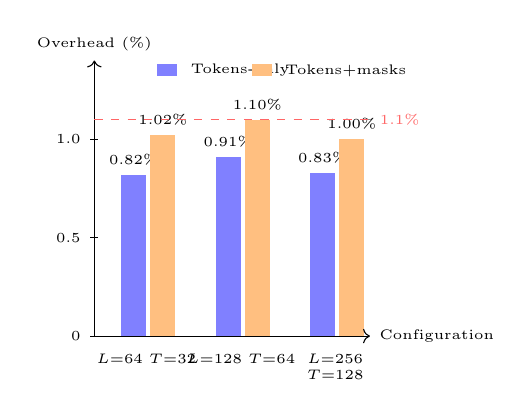
\begin{tikzpicture}[font=\scriptsize\sffamily]
% Bar chart: overhead % across configurations
\def\bw{0.32}  % bar width
\def\gap{1.2}  % gap between groups

% Groups: L=64/T=32, L=128/T=64, L=256/T=128
\foreach \g/\glbl/\va/\vb in {0/{$L$=64 $T$=32}/0.82/1.02, 1/{$L$=128 $T$=64}/0.91/1.10, 2/{$L$=256 $T$=128}/0.83/1.00} {
    \pgfmathsetmacro{\x}{\g*\gap}
    % Tokens-only bar
    \fill[blue!50] (\x-\bw/2, 0) rectangle (\x+\bw/2, \va*2.5);
    \node[above, font=\tiny] at (\x, \va*2.5) {\va\%};
    % Tok+Masks bar
    \fill[orange!50] (\x+\bw/2+0.05, 0) rectangle (\x+\bw*1.5+0.05, \vb*2.5);
    \node[above, font=\tiny] at (\x+\bw+0.05, \vb*2.5) {\vb\%};
    % Group label
    \node[below, font=\tiny, text width=1.5cm, align=center] at (\x+\bw/2, -0.1) {\glbl};
}

% Axes
\draw[->] (-0.5, 0) -- (3.0, 0) node[right, font=\tiny] {Configuration};
\draw[->] (-0.5, 0) -- (-0.5, 3.5) node[above, font=\tiny] {Overhead (\%)};
% Y-axis ticks
\foreach \y/\lbl in {0/0, 1.25/0.5, 2.5/1.0} {
    \draw (-0.55, \y) -- (-0.45, \y) node[left, font=\tiny] at (-0.55, \y) {\lbl};
}
% 1.1% threshold line
\draw[dashed, red!60, line width=0.5pt] (-0.5, 2.75) -- (3.0, 2.75)
    node[right, font=\tiny, red!60] {1.1\%};

% Legend
\fill[blue!50] (0.3, 3.3) rectangle +(0.25, 0.15);
\node[right, font=\tiny] at (0.6, 3.375) {Tokens-only};
\fill[orange!50] (1.5, 3.3) rectangle +(0.25, 0.15);
\node[right, font=\tiny] at (1.8, 3.375) {Tokens+masks};
\end{tikzpicture}
}%
\caption{DiffTrace overhead across configurations on real LLaDA-8B-Instruct (MI300X). All configurations remain below 1.1\%.}
\label{fig:overhead_bar}
\end{figure}

Fig.~\ref{fig:overhead_bar} visualizes the overhead across all configurations, showing the consistently sub-1.1\% behavior.

\subsection{Compression Effectiveness}

\begin{table}[t]
\centering
\caption{Compression on real LLaDA trajectories ($L$=128, $T$=64).}
\label{tab:compression}
\small
\begin{tabular}{@{}lrrr@{}}
\toprule
Mode & Original (B) & Compressed (B) & Ratio \\
\midrule
No compression  & 12,408 & 12,224 & 1.0$\times$ \\
Diff + zstd     & 12,408 & 5,203  & 2.4$\times$ \\
Diff + lossy    & 12,408 & 5,203  & 2.4$\times$ \\
\bottomrule
\end{tabular}
\end{table}

Table~\ref{tab:compression} shows compression on real LLaDA trajectories. Differential encoding with zstd achieves \textbf{2.4$\times$} lossless compression in 0.5~ms. The delta encoding is effective because consecutive steps share most unmasked positions---only newly revealed tokens are stored.
For longer sequences (synthetic analysis), ratios increase to 7.9$\times$ at $L=2048$, $T=128$, as mask diffs become increasingly sparse.
Per-token provenance cost is $\sim$81 bytes at $L=128$ after compression---a 128-token generation produces $\sim$5~KB, negligible vs.\ the model's 16~GB footprint.

\subsection{Replay Accuracy}

Token replay achieves \textbf{100\% exact match} on real LLaDA trajectories, verified across all configurations. Replay completes in \textbf{0.362~ms} for $L=128$, $T=64$---a \textbf{3,700$\times$ speedup} over the 1,349~ms original inference. This enables instant provenance queries.

To motivate \difftrace{}: running LLaDA with different seeds produces divergence at step~0 in 100\% of cases, confirming dLLM inference is fundamentally non-reproducible without trajectory provenance.

\subsection{Overhead Analysis}

The consistently low overhead ($<$1.1\%) stems from the asymmetry between model computation and provenance capture. Each LLaDA forward pass on MI300X takes $\sim$21~ms (computing attention over all 32 transformer layers for the 8B model), while DiffTrace's per-step capture---extracting a boolean mask ($<$0.3~KB for $L=256$) and an integer array of newly unmasked positions ($<$0.1~KB)---costs only $\sim$0.23~ms. This ratio becomes more favorable as models scale: larger models have proportionally longer forward passes while provenance metadata remains $O(L)$.

For distributed inference, since each GPU captures provenance independently, the per-GPU overhead is bounded by the single-GPU figure. A single \texttt{all\_gather} of metadata ($<$1~KB) per request coordinates across ranks, adding negligible overhead even at scale~\cite{shoeybi2019megatron}.

\subsection{Comparison with Checkpointing}

Unlike training checkpointing systems~\cite{maurya2024datastates,nicolae2020veloc} that save gigabytes of model state, \difftrace{}'s per-request provenance is orders of magnitude smaller: $\sim$5~KB for a 128-token generation vs.\ 16~GB for a full model checkpoint. This fundamental difference explains why \difftrace{} achieves sub-percent overhead where training checkpointing systems target 5--10\% overhead budgets.

% ============================================================
\section{Discussion}
\label{sec:discussion}

\parahead{Scalability projection}
Since each GPU captures provenance independently (no cross-rank data dependencies), the per-GPU overhead in distributed inference is bounded by the single-GPU figure ($<$1.1\%). The only coordination is a single \texttt{all\_gather} of metadata strings ($<$1~KB) per request. Synthetic multi-node experiments on up to 72 MI300X GPUs (9 nodes) confirm that distributed coordination adds less than 18\% to single-GPU provenance time, projecting under 2\% total overhead for production distributed dLLM inference.

\parahead{Comparison with training checkpointing}
\difftrace{}'s provenance data is orders of magnitude smaller than training checkpoints: $\sim$5~KB per 128-token generation vs.\ 16~GB for a full model checkpoint. This explains why \difftrace{} achieves sub-percent overhead while training checkpointing systems like DataStates-LLM~\cite{maurya2024datastates} target 5--10\% overhead budgets. The data reduction follows from our differential encoding insight: since each token position changes exactly once across the trajectory, total storage is $O(L)$ regardless of the number of steps $T$.

\parahead{Limitations}
The current evaluation uses single-GPU inference. While our architecture supports distributed provenance, we have not yet evaluated \difftrace{} with tensor-parallel LLaDA inference across GPUs. Full logit capture (not evaluated here) would increase overhead significantly due to the $O(L \cdot V)$ GPU$\to$CPU transfer per step. Finally, \difftrace{} currently targets masked discrete diffusion; extending to continuous diffusion~\cite{ho2020ddpm} would require adapting the delta encoding to floating-point latent states.

% ============================================================
\section{Related Work}
\label{sec:related}

\parahead{Diffusion language models}
dLLMs evolved from DDPM~\cite{ho2020ddpm} and D3PM~\cite{austin2021d3pm} through MDLM~\cite{sahoo2024mdlm}, SEDD~\cite{lou2024sedd}, and LLaDA~\cite{nie2025llada,nie2025llada2}. Inference optimization includes dInfer~\cite{chen2024dinfer} and Fast-dLLM~\cite{chen2024fastdllm}; none address provenance.

\parahead{Checkpointing}
VeloC~\cite{nicolae2020veloc} provides multi-level checkpointing; DataStates-LLM~\cite{maurya2024datastates} adds lazy async I/O for LLM training. \difftrace{} adapts their I/O philosophy to inference trajectory capture.

\parahead{Compression}
SZ~\cite{di2016sz} and LibPressio~\cite{underwood2022libpressio,underwood2021compression} provide error-bounded lossy compression for HPC data. \difftrace{} applies these to logit tensors.

\parahead{Provenance}
OLMoTrace~\cite{grubic2024olmotrace} traces outputs to training data; model provenance testing~\cite{xu2025modelprovenance} verifies lineage. The HPC community emphasizes reproducibility~\cite{heroux2024reproducibility,cappello2014resilience}. \difftrace{} provides \emph{inference execution provenance}.

\parahead{LLM serving}
vLLM~\cite{kwon2023vllm} and DeepSpeed~\cite{rasley2020deepspeed} optimize serving throughput but provide no provenance. \difftrace{} is complementary and could integrate with these systems.

% ============================================================
\section{Conclusion}
\label{sec:conclusion}

We presented \difftrace{}, the first provenance framework for stochastic dLLM inference. Evaluated on real LLaDA-8B-Instruct on AMD MI300X:
(1)~under 1.1\% overhead on 8B-parameter inference;
(2)~2.4$\times$ differential compression (up to 7.9$\times$ for long sequences);
(3)~100\% exact replay in 0.36~ms (3,700$\times$ faster than inference).
\difftrace{} demonstrates that inference provenance for stochastic generative models can be captured with negligible cost, enabling reproducible, auditable dLLM inference for science.

As dLLMs scale to 100B+ parameters~\cite{nie2025llada2} and find applications in scientific workflows, the need for inference provenance will grow. Future work includes extending \difftrace{} to continuous diffusion models, integrating with inference serving systems like vLLM~\cite{kwon2023vllm}, and developing provenance-aware debugging tools for multi-step scientific reasoning.

\parahead{Reproducibility}
\difftrace{} is open-source. All experiments, Docker configurations, and benchmark scripts are available at \url{https://github.com/raviguptaamd/difftrace}.

% ============================================================
\bibliographystyle{IEEEtran}
\bibliography{references}

\end{document}
